%!TEX encoding = UTF-8 Unicode
%!TEX root = ../compendium.tex

\chapter{Virtuell maskin}\label{appendix:vbox}

\section{Vad är en virtuell maskin?}

Du kan köra alla kursens verktyg i en så kallad \textbf{virtuell maskin} (förk. vm, eng. \textit{virtual machine}). 
Detta är ett enkelt och säkert sätt köra ett annat operativsystem i en ''sandlåda'' som inte påverkar din dators ursprungliga operativsystem. Figur \ref{fig:vm} visar kursens virtuella maskin med sin exklusiva bakgrundsbild. Exekveringen av en vm sker på en \textbf{värddator} \Eng{host}. I figur \ref{fig:vm} körs kursens vm i en Linux-värd med virtualiseringsapplikationen \textit{VirtualBox}\footnote{\href{https://en.wikipedia.org/wiki/VirtualBox}{/en.wikipedia.org/wiki/VirtualBox}}, som är öppen och gratis och även finns för Windows- och macOS-värdar. 



\begin{figure}[H]
\centering
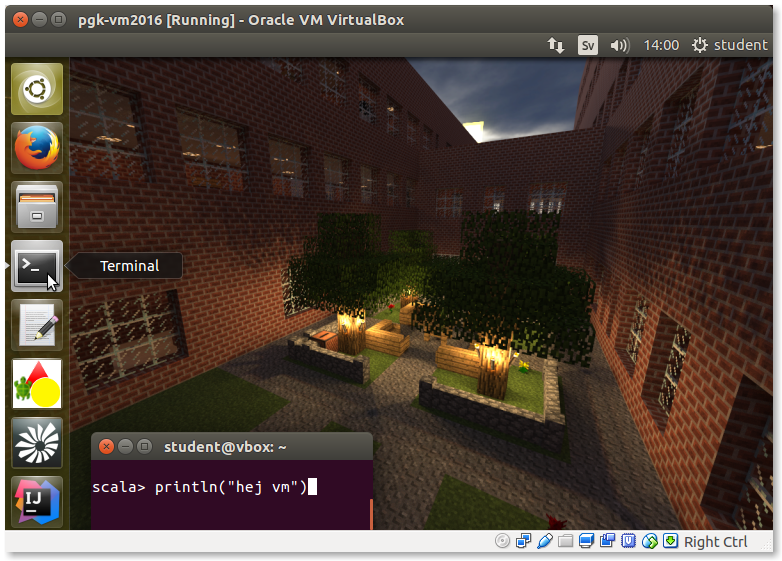
\includegraphics[width=1.0\textwidth]{../img/vm.png}
\caption{Den virtuella maskinen pgk-vm2016.}
\label{fig:vm}
\end{figure}


\section{Vad innehåller kursens vm?}

Kursens virtuell maskin har alla verktyg som du behöver förinstallerade.  Vår vm kör Ubuntu 16.04.1 med fönstermiljön Unity, vilket är samma miljö som körs på Linuxdatorerna i E-huset på LTH. 

Detta och mycket annat är förinstallerat i kursens vm:

\begin{itemize}
\item \texttt{java} och \texttt{javac} med JDK 8
\item \texttt{scala} och \texttt{scalac} med Scala 2.11.8
\item Kojo 2.4.09
\item Eclipse Mars.2 med ScalaIDE 4.4.1
\item InteliJ IDEA 2016.2 med Scala-plugin
\item \texttt{gedit}
\item \texttt{git}
\item \texttt{sbt}
\item \texttt{pdflatex} (inkl. texlive-full, texlive-lang-europe, texworks, m.m.) 
\item \texttt{amm} 0.7.0, för Scala-skriptning, se \url{http://www.lihaoyi.com/Ammonite/}
\item Alla skrivbordsappar som kommer med Unbuntu, t.ex. LibreOffice för ordbehandling och kalkylblad  kompatibel med MS Word och MS Excel.  
\item Kursens repo i katalogen \code{~/git/lunduniversity/introprog/} inklusive  \texttt{compendium/compenium.pdf} och kursens \texttt{workspace}.
\item Den maximalt avskalade fönstermiljön \url{https://i3wm.org/} om du gillar att jobba effektivt med tangentbordskortkommandon. Logga först ut genom att klicka i systemmenyn längst uppe till höger och välj sedan i3 i rullgardingsmenyn som trillar ner när du klickar på Ubuntu-symbolen ovanför lösenordsrutan på inloggningsskärmen.
\end{itemize}

\section{Installera kursens vm}

Det går lite långsammare att köra i en virtuell maskin jämfört med att köra direkt ''på metallen'', då det sker vissa översättningar och kontroller under virtualiseringsprocessen som annars är onödiga. Och den virtuella maskinen behöver få en rejäl andel av din dators minne. Så för att köra en virtuell maskin utan att det ska bli segt behövs en ganska snabb processor, gärna över 2.5 GHz, och ganska mycket minne, gärna mer än 4GB. 

Även om det går lite segt är en virtuell maskin ett utmärkt sätt att prova på Linux och Ubuntu. Eftersom man lätt kan spara undan en hel maskin är det ett bra sätt att experimentera med olika inställningar och installationer utan att ens normala miljö påverkas. Och kör du terminalfönster och en enkel editor brukar svag prestanda och lite minne inte vara ett stort problem.\footnote{Om du tycker det går alltför segt kan du istället installera Linux direkt på din dator jämsides ditt andra operativsystem -- fråga någon som vet om hur man gör detta.} 

Gör så här för att installera VirtualBox och köra kursens virtuella maskin:
\begin{enumerate}
\item  Ladda ner VirtualBox v5 för ditt operativsystem här och installera: \\ \url{https://www.virtualbox.org/wiki/Downloads}

\item Ladda även ner \textit{''VirtualBox Oracle VM VirtualBox Extension Pack''}  och installera enligt instruktionerna här:\\ \url{https://www.virtualbox.org/wiki/Downloads} \\ Om du stöter på problem eller undrar hur, fråga någon om hjälp.

\item Det kan hända att du får felmeddelande som innehåller något som liknar ''Intel VT-x'' eller ''Hyper-V'', så som beskrivs här:
\\ \href{http://www.howtogeek.com/213795/how-to-enable-intel-vt-x-in-your-computers-bios-or-uefi-firmware/}{www.howtogeek.com/213795/how-to-enable-intel-vt-x-in-your-computers-bios-or-uefi-firmware}\\
Då behöver du tillåta virtualiseringsfunktioner i BIOS på din dator. Om du inte vet hur du ska göra detta, be någon som vet om hjälp.

\item     Ladda ner filen \texttt{pgk-vm2016.ova} här: \\ \url{http://fileadmin.cs.lth.se/pgk/pgk2016.ova} \\ OBS! Då filen är på nästan 10GB kan nedladdningen ta \textit{mycket} lång tid, kanske flera timmar beroende på din internetuppkoppling. Har du problem med nedladdningstider kan du prova att ladda ner filen till ett USB-minne på skolans datorer, så att nedladdningen sker lokalt i E-huset.

\item     Öppna VirtualBox och välj \MenuArrow{File}\Menu{Import appliance..} och bläddra till filen \code{pgk-vm2016.ova} och klicka \Button{Next} och sedan \Button{Import}. Själva importen kan ta lång tid, kanske flera tiotals minuter beroende på hur snabbt din dator läser från disk.

\item Markera maskinen \textbf{pgk-vm2016} och välj menyn \MenuArrow{Machine}\Menu{Settings...} (eller tryck Ctrl+S) och undersök inställningarna. Se speciellt under fliken \textbf{System} och \textbf{Motherboard} där det står hur mycket \textbf{Base memory} du tilldelar. Om du har gott om minne kan du med fördel öka minnet till 4096MB, speciellt om du tänker köra igång de tungkörda IDE-apparna Eclipse eller IntelliJ.

\item Starta maskinen \textbf{pgk-vm2016} med ett dubbelklick. Ha lite tålamod innan maskinen är igång. Du kan behöva justera skärmstorleken i värdmaskinsmenyn \Menu{View}.

\item Öppna ett terminalfönster och skriv \texttt{scala} och du är igång och kan börja göra övningarna i detta kompendium!

\item Du behöver inte logga in för att köra igång maskinen under användaren \code{student}, men du  behöver lösenordet\footnote{\code{pgkBytMig2016}} för att installera nya program.

\item Börja med att uppdatera mjukvaran på din virtuella maskin genom att köra dessa terminalkommando:
\begin{REPLnonum}
$ sudo apt-get update
$ sudo apt-get upgrade
$ sudo apt-get dist-upgrade
\end{REPLnonum}


\item För att dra ner de senaste inlämningarna i kursrepot och uppdatera kompendiet och workspace, kör följande terminalkommando:
\begin{REPLnonum}
$ cd ~/git/lunduniversity/introprog
$ git pull
$ sbt build
$ sbt eclipse
\end{REPLnonum}

\item Om allt verkar fungera fint kan du nu prova att sätta på 3D-accelereringen för snabbare grafikrendering. Stäng maskinen genom att välja \Menu{Shut Down...} i systemmenyn. Ändra inställningar i menyn \MenuArrow{Settings...}\Menu{Display} genom att i fliken \textbf{Acceleration} under \textbf{Screen} markera \FramedCheckmark{Enable 3D acceleration}. Stara maskinen. Om det fungerar så blir animeringar avsevärt snyggare och smidigare. Om det inte fungerar, stäng av maskinen med \Menu{Power off} och avmarkera \FramedUnchecked{Enable 3D acceleration} igen.\footnote{Du kan också prova att genomföra stegen som visas här, för att ominstallera vissa saker som kan ha uppdaterats sedan detta skrevs: \url{https://www.linuxbabe.com/virtualbox/how-to-install-virtualbox-guest-additions-on-ubuntu-step-by-step}}

\end{enumerate}